% \chapter{System Overview and Data Pipeline}
% \label{chap:pipeline}

% This chapter describes the end-to-end pipeline that turns raw Indian
% court-judgment text into a labelled, leakage-audited, heterogeneous
% knowledge graph ready for Graph Neural Network (GNN) training. The
% pipeline was designed around three practical constraints: (i) the corpus
% is large and noisy, so every stage is a batch process with explicit
% caching and auditing; (ii) many of the signals a predictor would want
% (decisions, dispositions, operative paragraphs) are precisely the signals
% a legally honest experiment must remove, so leakage prevention has to be
% baked in rather than bolted on; and (iii) the downstream target is a
% graph, so text extraction and entity resolution have to produce outputs
% that can be reified as typed nodes and edges without lossy renormalisation
% later on.

% \section{System Architecture Overview}

% The system is organised as a six-stage pipeline. Each stage is an
% independently re-runnable batch process; intermediate artefacts are
% cached on disk so that an expensive step (OpenNyAI NER on tens of
% thousands of judgments, or bge-m3 embedding on millions of text spans)
% never has to be repeated when a later stage changes.

% \begin{figure}[H]
%   \centering
%   \begin{tikzpicture}[
%       node distance=0.45cm and 0.7cm,
%       every node/.style={font=\small},
%       stage/.style={rectangle, rounded corners, draw=black!70, thick,
%         fill=blue!6, minimum width=4.2cm, minimum height=0.95cm,
%         align=center, text width=4.1cm},
%       artefact/.style={rectangle, draw=black!40, dashed, fill=gray!4,
%         minimum width=4.2cm, minimum height=0.7cm, align=center,
%         text width=4.1cm, font=\footnotesize\itshape},
%       arrow/.style={-{Stealth[length=2mm]}, thick}
%     ]
%     \node[stage] (s1) {\textbf{1. Document Collection}\\raw judgment
%       \texttt{.txt} files};
%     \node[artefact, below=of s1] (a1) {per-bucket raw corpora
%       (5 legal domains)};
%     \node[stage, below=of a1] (s2) {\textbf{2. OpenNyAI NER + RR}\\
%       Legal NER, Rhetorical Roles, Summariser};
%     \node[artefact, below=of s2] (a2) {enriched JSON: annotated spans,
%       RR labels, summary};
%     \node[stage, below=of a2] (s3) {\textbf{3. Mistral Outcome
%       Labelling}\\case-level win/loss/neutral + score};
%     \node[artefact, below=of s3] (a3) {\texttt{*\_timed\_mistral}
%       case JSONs};
%     \node[stage, right=3.2cm of s1] (s4) {\textbf{4. Multi-Hearing
%       Merging}\\fold earlier hearings into the final decision};
%     \node[artefact, below=of s4] (a4) {\texttt{*\_MERGED.json} final
%       case records};
%     \node[stage, below=of a4] (s5) {\textbf{5. Leakage-Safe
%       Cleaning}\\drop decision fields, mask phrases, filter RR labels};
%     \node[artefact, below=of s5] (a5) {cleaned
%       \texttt{CleanedCase} objects};
%     \node[stage, below=of a5] (s6) {\textbf{6. Graph Construction +
%       bge-m3 Encoding}\\PyG \texttt{HeteroData} + text embeddings};
%     \node[artefact, below=of s6] (a6) {per-bucket + cross-bucket
%       graph caches};
%     \draw[arrow] (s1) -- (a1);
%     \draw[arrow] (a1) -- (s2);
%     \draw[arrow] (s2) -- (a2);
%     \draw[arrow] (a2) -- (s3);
%     \draw[arrow] (s3) -- (a3);
%     \draw[arrow] (a3.east) -- ++(0.8,0) |- (s4.west);
%     \draw[arrow] (s4) -- (a4);
%     \draw[arrow] (a4) -- (s5);
%     \draw[arrow] (s5) -- (a5);
%     \draw[arrow] (a5) -- (s6);
%     \draw[arrow] (s6) -- (a6);
%   \end{tikzpicture}
%   \caption{The six-stage data pipeline. Solid boxes are processing
%   stages; dashed boxes are cached on-disk artefacts that feed the next
%   stage.}
%   \label{fig:pipeline}
% \end{figure}

% Stages~1--3 are \emph{textual enrichment}: they turn plain text into a
% structured JSON record with entities, rhetorical-role spans, and a
% case-level outcome label. Stage~4 reconciles the fact that a single
% legal matter often produces multiple hearing documents, so that each
% final case corresponds to one legal dispute rather than one PDF. Stage~5
% is a leakage-safety gate: it explicitly removes the fields, sections,
% and phrases that would let a model trivially recover the outcome.
% Stage~6 reifies the cleaned records as a typed heterogeneous graph and
% attaches pre-computed \texttt{bge-m3} text embeddings to every text
% node. Chapter~\ref{chap:kg} details the schema produced by stage~6.

% \section{Document Collection and Legal Domains}

% \emph{(Document collection methodology -- sources, filters, deduplication
% -- to be described in a later revision.)}

% The collected corpus is organised into five \textbf{legal domain
% buckets}, chosen so that each bucket is large enough to train a
% domain-specific graph and internally coherent in terms of statutory
% framework, party structure, and typical remedies. The buckets are:

% \begin{itemize}
%   \item \textbf{Family \& Matrimonial} (\texttt{family\_matrimonial\_timed\_mistral}):
%     matrimonial disputes, maintenance, custody, and dowry-related
%     proceedings. Dominated by IPC~498A, Sections~482, 506, and the CrPC.
%   \item \textbf{Financial Fraud} (\texttt{fin\_fraud\_timed\_mistral}):
%     cheating, forgery, dishonour, and economic offences. Dominated by
%     IPC~420, 468, 471.
%   \item \textbf{Land \& Property} (\texttt{land\_property\_timed\_mistral}):
%     land acquisition, title, and property disputes. Dominated by the
%     Land Acquisition Act~1894 and the Constitution of India.
%   \item \textbf{Motor Accidents} (\texttt{motor\_accidents\_timed\_mistral}):
%     compensation claims and related appeals. Dominated by the Motor
%     Vehicles Act~1988 and Section~166.
%   \item \textbf{Sexual Offences} (\texttt{sexual\_offences\_timed\_mistral}):
%     offences against the person, including POCSO matters. Dominated by
%     the IPC, CrPC, and POCSO Act.
% \end{itemize}

% Every downstream artefact -- entity canonicalisation tables,
% rhetorical-role annotations, outcome labels, and graph caches -- is
% produced both per bucket and in a unified \emph{cross-bucket} view.
% This two-level organisation is what later makes cross-domain transfer
% and cross-bucket bridge analysis possible
% (Chapter~\ref{chap:graph_exploration}).

% \section{Named Entity Recognition and Rhetorical Role Classification}

% \subsection{The OpenNyAI Pipeline}

% Textual enrichment is performed with the OpenNyAI legal NLP stack,
% running locally on GPU. The production configuration uses:

% \begin{itemize}
%   \item \texttt{Legal NER} with
%     \texttt{ner\_model\_name="en\_legal\_ner\_trf"}, sentence-level
%     inference (\texttt{ner\_do\_sentence\_level=True}) and the built-in
%     post-processor (\texttt{ner\_do\_postprocess=True});
%   \item \texttt{Rhetorical\_Role} classification, assigning each
%     sentence a legal discourse label (\textsc{Preamble}, \textsc{Facts},
%     \textsc{Arguments}, \textsc{Ratio}, \textsc{RPC}, etc.);
%   \item \texttt{Summarizer} executed after rhetorical-role
%     classification, which produces the section-structured summary
%     (\textsc{Preamble}, \textsc{facts}, \textsc{arguments}, and a
%     decision block that is later discarded).
% \end{itemize}

% The environment is pinned (spaCy~3.2.4, pydantic~1.7.4,
% CUDA-enabled PyTorch and CuPy) and run GPU-only: silent CPU fallback is
% disabled so that a broken GPU configuration fails fast rather than
% silently degrading throughput. All model caches are redirected into
% project-local folders so that re-runs do not contaminate
% \texttt{\$HOME}. Each input judgment yields a combined JSON with NER
% annotations, rhetorical-role spans, and the summary.

% \subsection{Entity Types and Their Graph Roles}

% OpenNyAI's legal NER tags span several coarse types; the ones we reify
% as graph nodes are:

% \begin{itemize}
%   \item \textsc{Statute} and \textsc{Provision} -- statutes (e.g.\ IPC,
%     CrPC, Motor Vehicles Act) and their sections (e.g.\ Section~482).
%     Provisions are additionally linked to their parent statute via a
%     \texttt{belongs\_to\_statute} edge.
%   \item \textsc{Precedent} -- cited case references.
%   \item \textsc{Court} and \textsc{Judge} -- the court the matter is
%     heard in and the presiding bench.
%   \item \textsc{Petitioner}, \textsc{Respondent},
%     \textsc{Petitioner\_Lawyer}, \textsc{Defence\_Lawyer},
%     \textsc{Lawyer} -- typed party and counsel roles. Role assignment
%     uses the section in which the mention first appears (preamble vs.\
%     argument blocks) combined with OpenNyAI's entity labels.
%   \item \textsc{Org}, \textsc{GPE}, \textsc{Date}, \textsc{Case\_Number}
%     -- auxiliary types extracted by NER, retained in the cleaned JSON
%     but excluded from the final reasoning-focused graph
%     (Section~\ref{sec:graph_schema}).
% \end{itemize}

% Entities are canonicalised per bucket: surface forms are normalised
% (case, whitespace, punctuation), grouped, and re-projected as
% \texttt{canonical\_name}. Canonicalisation is what allows the same
% statute or court to be a \emph{single shared node} across the thousands
% of cases that mention it, which is the structural property that makes
% the graph useful for cross-case reasoning.

% \subsection{Rhetorical Role Taxonomy and Leakage-Safe Filtering}

% OpenNyAI's rhetorical-role taxonomy is the hinge on which the
% leakage-safety story turns. Of the labels produced by the RR model, two
% are inherently decisive -- \textbf{RPC} (Ratio and Precedent Cited, in
% practice the court's operative paragraph) and \textbf{RLC} (Ruling by
% Lower Court). Keeping either of them would let a classifier read the
% outcome verbatim.

% The cleaning stage therefore treats both labels as
% \texttt{FORBIDDEN\_ANNOTATION\_LABELS}: any annotation whose label set
% intersects \{\textsc{RPC}, \textsc{RLC}\} is dropped outright, along
% with any annotation whose summary section is \textsc{decision} or whose
% label string contains \texttt{"decision"}, \texttt{"disposition"},
% \texttt{"operative"}, \texttt{"order"}, or \texttt{"rpc"}. Only the
% three non-decisive summary fields -- \textsc{Preamble},
% \textsc{facts}, and \textsc{arguments} -- are retained as text sources
% for the graph's text nodes. This is the first leakage gate; a second,
% phrase-level gate is described in Section~\ref{sec:leakage_prevention}.

% \section{Outcome Labelling with Mistral}

% \subsection{Labelling Methodology}

% Case-level outcome labels are produced by prompting a Mistral LLM with
% the OpenNyAI summary and asking it to return a structured judgement:
% a label ($\text{win} = +1$, $\text{loss} = -1$, or \textsc{neutral}),
% a confidence-weighted \texttt{outcome\_score} in $[-1, +1]$, and a short
% textual explanation. Labelling is done from the \emph{summaries
% produced by OpenNyAI}, not from the raw judgment text, so that the
% label generator sees the same content the downstream model would see
% if no leakage cleaning were applied -- which then forces us to remove
% the decision-bearing portions of that summary before training. The
% resulting artefacts are the \texttt{*\_timed\_mistral} buckets used
% throughout the rest of the thesis.

% Both single-label and multi-label variants are produced
% (\texttt{add\_case\_outcome\_labels\_mistral.py} and
% \texttt{add\_multi\_label\_outcome\_from\_enriched.py}). This work uses
% the single-label variant as the prediction target; the multi-label
% variant is kept as a diagnostic artefact.

% \subsection{Coverage and Label Distribution}

% Labelling coverage and the resulting win/loss/neutral distribution are
% summarised in Figures~\ref{fig:labelling_coverage}
% and~\ref{fig:outcome_distribution}. Coverage is near-complete across
% all five buckets; the class distribution is moderately imbalanced
% (roughly $60\%$ \textsc{win} to $40\%$ \textsc{loss} on the pooled
% cross-bucket dataset), which motivates the use of macro-F1 alongside
% accuracy as a primary metric in Chapter~\ref{chap:results}.

% \begin{figure}[H]
%   \centering
%   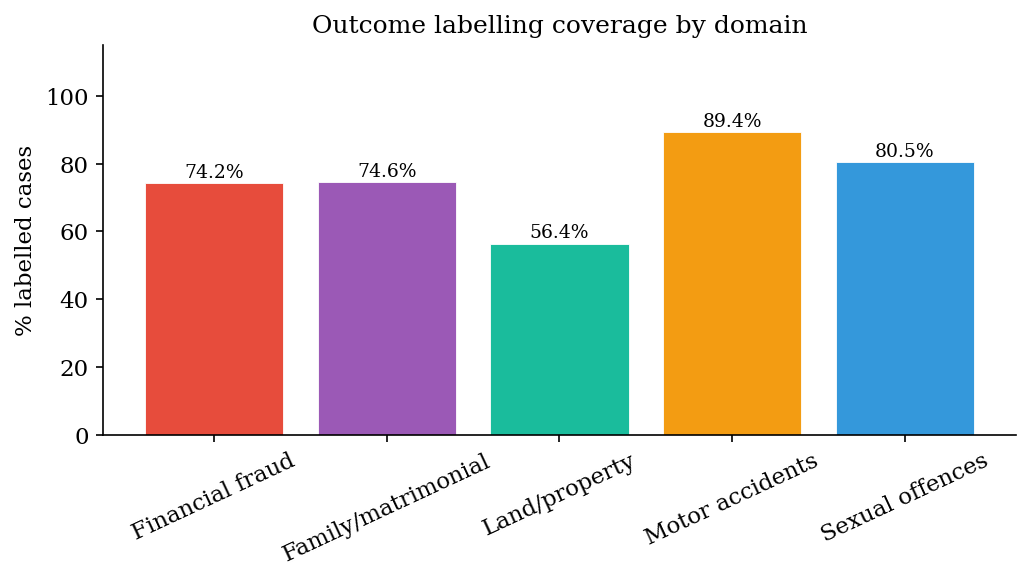
\includegraphics[width=0.92\textwidth]{figures/labelling_coverage_full.png}
%   \caption{Mistral labelling coverage per bucket.}
%   \label{fig:labelling_coverage}
% \end{figure}

% \begin{figure}[H]
%   \centering
%   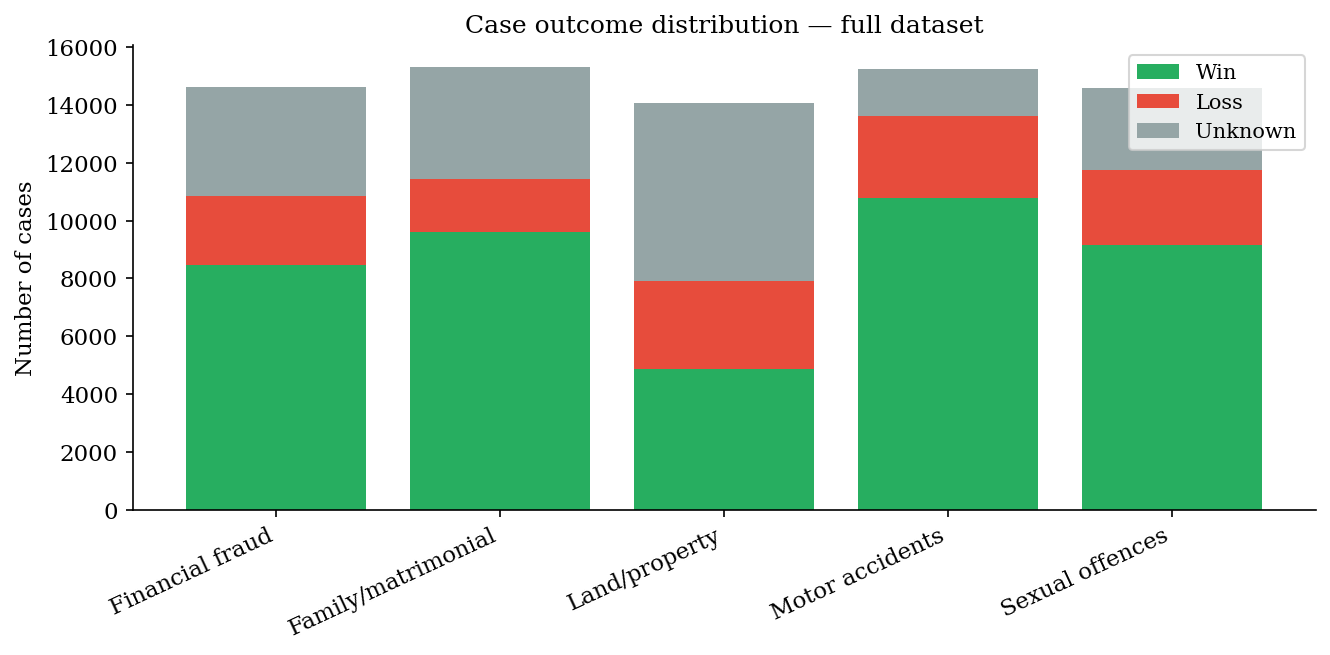
\includegraphics[width=0.92\textwidth]{figures/outcome_distribution_full.png}
%   \caption{Outcome label distribution per bucket.}
%   \label{fig:outcome_distribution}
% \end{figure}

% \section{Multi-Hearing Merging}
% \label{sec:multi_hearing_merging}

% \subsection{The Problem}

% A single legal matter frequently produces more than one judgment
% document: interim orders, remands, partial disposals, and the final
% decision may all be published as separate PDFs with distinct
% Indian-Kanoon-style filenames that nonetheless refer to the same case.
% If these hearing files are fed into the graph independently, three
% things go wrong:

% \begin{enumerate}
%   \item duplicate \textsc{Case} nodes for what is actually one dispute
%     inflate the node count and double-count outcomes;
%   \item the outcome label of the final hearing is not propagated to the
%     earlier hearings, so the training signal is noisy; and
%   \item cross-case structural signals (shared parties, statutes, and
%     counsel across hearings) are double-counted as if they were
%     independent observations.
% \end{enumerate}

% \subsection{Merge Strategy}

% The merging pipeline lives under
% \texttt{Thesis\_FINAL\_DATA/TIMELINE} and
% \texttt{DATA\_SET\_BUILDER\_AND\_EXPLORER/Timeline\_Maker}. Per bucket,
% filenames are parsed into a \texttt{(title,\ hearing\_date)} tuple; the
% latest hearing becomes the \emph{final} case, and every older hearing
% with the same title is \emph{folded} into that final case's JSON. The
% fold step either appends the older document's text under a
% \texttt{prior\_hearings} block (when the final document does not
% already contain that text) or is skipped when the final document
% already subsumes it. Every merge is logged in a per-bucket
% \texttt{report.json} so the operation is auditable and reversible.

% The scale of the fold is non-trivial but concentrated:

% \begin{table}[H]
%   \centering
%   \small
%   \begin{tabular}{lrrrrr}
%     \toprule
%     Bucket & Inputs & Final cases & Folded in & Appended & Already contained \\
%     \midrule
%     Family \& Matrimonial & 15{,}800 & 15{,}306 & 493 & 490 & 3 \\
%     Financial Fraud & 15{,}014 & 14{,}615 & 399 & 396 & 3 \\
%     Land \& Property & 14{,}324 & 14{,}051 & 251 & 242 & 9 \\
%     Motor Accidents & 15{,}271 & 15{,}236 & 32 & 30 & 2 \\
%     Sexual Offences & 15{,}532 & 14{,}596 & 936 & 932 & 4 \\
%     \midrule
%     \textbf{Total} & \textbf{75{,}941} & \textbf{73{,}804} & \textbf{2{,}111}
%       & \textbf{2{,}090} & \textbf{21} \\
%     \bottomrule
%   \end{tabular}
%   \caption{Multi-hearing merge statistics. 2{,}111 older hearing
%   documents across the five buckets were folded into 2{,}090 merged
%   final-case JSONs; the remaining 21 were already fully contained in
%   the final hearing.}
%   \label{tab:merge_stats}
% \end{table}

% Sexual-offences matters fold most aggressively, which is consistent with
% their tendency to generate multiple remand and bail-stage orders before
% a final judgment; motor-accidents matters fold least, because the
% compensation process terminates in one tribunal order more often than
% it does in the other buckets.

% \section{Technology Stack}

% The pipeline is entirely Python-based. NER, RR, and summarisation run
% on top of \texttt{opennyai} with spaCy~3.2.4 and CUDA-enabled PyTorch
% and CuPy, provisioned via the pinned micromamba environment
% \texttt{fixed\_gpu\_opennyai\_final}. Outcome labelling uses a Mistral
% model invoked through a batched client script. Multi-hearing merging is
% implemented with \texttt{merge\_cases.py} and \texttt{merge\_cases\_v2.py}
% under the \texttt{Timeline\_Maker} module. Graph construction is built
% on \texttt{torch\_geometric}'s \texttt{HeteroData}, with text
% embeddings produced by the \texttt{BAAI/bge-m3} sentence-transformer
% model running multi-process on GPU and cached per bucket. Training,
% ablation, and analysis scripts live under the \texttt{section\_GNN}
% module.

\chapter{System Overview and Data Pipeline}
\label{chap:pipeline}

This chapter describes the end-to-end pipeline that turns raw Indian
court-judgment text into a labelled, leakage-audited, heterogeneous
knowledge graph ready for Graph Neural Network (GNN) training. The
pipeline was designed around three practical constraints: (i) the corpus
is large and noisy, so every stage is a batch process with explicit
caching and auditing; (ii) many of the signals a predictor would want
(decisions, dispositions, operative paragraphs) are precisely the signals
a legally honest experiment must remove, so leakage prevention has to be
baked in rather than bolted on; and (iii) the downstream target is a
graph, so text extraction and entity resolution have to produce outputs
that can be reified as typed nodes and edges without lossy renormalisation
later on.

\section{System Architecture Overview}

The system is organised as a six-stage pipeline. Each stage is an
independently re-runnable batch process; intermediate artefacts are
cached on disk so that an expensive step (OpenNyAI NER on tens of
thousands of judgments, or bge-m3 embedding on millions of text spans)
never has to be repeated when a later stage changes.

\begin{figure}[H]
  \centering
  \begin{tikzpicture}[
      node distance=0.45cm and 0.7cm,
      every node/.style={font=\small},
      stage/.style={rectangle, rounded corners, draw=black!70, thick,
        fill=blue!6, minimum width=4.2cm, minimum height=0.95cm,
        align=center, text width=4.1cm},
      artefact/.style={rectangle, draw=black!40, dashed, fill=gray!4,
        minimum width=4.2cm, minimum height=0.7cm, align=center,
        text width=4.1cm, font=\footnotesize\itshape},
      arrow/.style={-{Stealth[length=2mm]}, thick}
    ]
    \node[stage] (s1) {\textbf{1. Document Collection}\\raw judgment
      \texttt{.txt} files};
    \node[artefact, below=of s1] (a1) {per-bucket raw corpora
      (5 legal domains)};
    \node[stage, below=of a1] (s2) {\textbf{2. OpenNyAI NER + RR}\\
      Legal NER, Rhetorical Roles, Summariser};
    \node[artefact, below=of s2] (a2) {enriched JSON: annotated spans,
      RR labels, summary};
    \node[stage, below=of a2] (s3) {\textbf{3. Mistral Outcome
      Labelling}\\case-level win/loss/neutral + score};
    \node[artefact, below=of s3] (a3) {\texttt{*\_timed\_mistral}
      case JSONs};
    \node[stage, right=3.2cm of s1] (s4) {\textbf{4. Multi-Hearing
      Merging}\\fold earlier hearings into the final decision};
    \node[artefact, below=of s4] (a4) {\texttt{*\_MERGED.json} final
      case records};
    \node[stage, below=of a4] (s5) {\textbf{5. Leakage-Safe
      Cleaning}\\drop decision fields, mask phrases, filter RR labels};
    \node[artefact, below=of s5] (a5) {cleaned
      \texttt{CleanedCase} objects};
    \node[stage, below=of a5] (s6) {\textbf{6. Graph Construction +
      bge-m3 Encoding}\\PyG \texttt{HeteroData} + text embeddings};
    \node[artefact, below=of s6] (a6) {per-bucket + cross-bucket
      graph caches};
    \draw[arrow] (s1) -- (a1);
    \draw[arrow] (a1) -- (s2);
    \draw[arrow] (s2) -- (a2);
    \draw[arrow] (a2) -- (s3);
    \draw[arrow] (s3) -- (a3);
    \draw[arrow] (a3.east) -- ++(0.8,0) |- (s4.west);
    \draw[arrow] (s4) -- (a4);
    \draw[arrow] (a4) -- (s5);
    \draw[arrow] (s5) -- (a5);
    \draw[arrow] (a5) -- (s6);
    \draw[arrow] (s6) -- (a6);
  \end{tikzpicture}
  \caption{The six-stage data pipeline. Solid boxes are processing
  stages; dashed boxes are cached on-disk artefacts that feed the next
  stage.}
  \label{fig:pipeline}
\end{figure}

Stages~1--3 are \emph{textual enrichment}: they turn plain text into a
structured JSON record with entities, rhetorical-role spans, and a
case-level outcome label. Stage~4 reconciles the fact that a single
legal matter often produces multiple hearing documents, so that each
final case corresponds to one legal dispute rather than one PDF. Stage~5
is a leakage-safety gate: it explicitly removes the fields, sections,
and phrases that would let a model trivially recover the outcome.
Stage~6 reifies the cleaned records as a typed heterogeneous graph and
attaches pre-computed \texttt{bge-m3} text embeddings to every text
node. Chapter~\ref{chap:kg} details the schema produced by stage~6.

\section{Document Collection and Legal Domains}

{\color{blue}
\subsection{Source Selection and Crawling Strategy}

The data source for the underlying judgments is Indian Kanoon (\texttt{indiankanoon.org}). It was selected for its comprehensive, publicly accessible archive of Indian High Court judgments and its semi-structured search interface, which is uniquely suited for programmatic access compared to proprietary databases. However, accessing a deep, historical sample from the platform involves structural challenges. Indian Kanoon's search results for any single query are practically truncated at a cap of 40 pages (approximately 400 accessible documents) per search window. 

To overcome this truncation, data collection was structured around discrete \emph{court-month windows}. For each target High Court and for each calendar month across the target years, the scraper executed an explicitly bounded query (e.g., \texttt{doctypes:<court> fromdate:1-<month>-<year> todate:<last\_day>-<month>-<year>}). By narrowing the temporal bounds to a single month per jurisdiction, the total number of judgments returned per window consistently stayed within the access limits, allowing for an exhaustive download of the raw corpus without relying on single broad keyword queries. The judgments were initially collected and stored directly in their raw PDF format. Furthermore, no deduplication methodologies were employed on the text or case level beyond a basic check to prevent re-downloading the same numeric Indian Kanoon document ID. 

\subsection{Local Bucketing and Legal Domains}

Rather than trusting black-box search engines to selectively define the corpus---which could bias the dataset towards heavily-cited ``landmark'' cases while omitting routine baseline cases---the classification of documents into specific legal domains was implemented locally as a deterministic post-processing step.

After downloading the entire accessible window, each raw PDF underwent text extraction (via PyMuPDF) and was passed through a local filtering script. This script evaluated the text against a rigid set of regular expressions corresponding to required statutory provisions (e.g., ``Section 498A IPC'', ``Motor Vehicles Act'', ``POCSO'') and contextual keyword constraints. Scraped texts that successfully matched a domain's predefined rules were partitioned into the respective local directory buckets.

The collected corpus resulting from this process is organised into five \textbf{legal domain buckets}, chosen so that each bucket is large enough to train a domain-specific graph and internally coherent in terms of statutory framework, party structure, and typical remedies. The buckets are:
}

\begin{itemize}
  \item \textbf{Family \& Matrimonial} (\texttt{family\_matrimonial\_timed\_mistral}):
    matrimonial disputes, maintenance, custody, and dowry-related
    proceedings. Dominated by IPC~498A, Sections~482, 506, and the CrPC.
  \item \textbf{Financial Fraud} (\texttt{fin\_fraud\_timed\_mistral}):
    cheating, forgery, dishonour, and economic offences. Dominated by
    IPC~420, 468, 471.
  \item \textbf{Land \& Property} (\texttt{land\_property\_timed\_mistral}):
    land acquisition, title, and property disputes. Dominated by the
    Land Acquisition Act~1894 and the Constitution of India.
  \item \textbf{Motor Accidents} (\texttt{motor\_accidents\_timed\_mistral}):
    compensation claims and related appeals. Dominated by the Motor
    Vehicles Act~1988 and Section~166.
  \item \textbf{Sexual Offences} (\texttt{sexual\_offences\_timed\_mistral}):
    offences against the person, including POCSO matters. Dominated by
    the IPC, CrPC, and POCSO Act.
\end{itemize}

Every downstream artefact -- entity canonicalisation tables,
rhetorical-role annotations, outcome labels, and graph caches -- is
produced both per bucket and in a unified \emph{cross-bucket} view.
This two-level organisation is what later makes cross-domain transfer
and cross-bucket bridge analysis possible
(Chapter~\ref{chap:graph_exploration}).

\section{Named Entity Recognition and Rhetorical Role Classification}

\subsection{The OpenNyAI Pipeline}

Textual enrichment is performed with the OpenNyAI legal NLP stack,
running locally on GPU. The production configuration uses:

\begin{itemize}
  \item \texttt{Legal NER} with
    \texttt{ner\_model\_name="en\_legal\_ner\_trf"}, sentence-level
    inference (\texttt{ner\_do\_sentence\_level=True}) and the built-in
    post-processor (\texttt{ner\_do\_postprocess=True});
  \item \texttt{Rhetorical\_Role} classification, assigning each
    sentence a legal discourse label (\textsc{Preamble}, \textsc{Facts},
    \textsc{Arguments}, \textsc{Ratio}, \textsc{RPC}, etc.);
  \item \texttt{Summarizer} executed after rhetorical-role
    classification, which produces the section-structured summary
    (\textsc{Preamble}, \textsc{facts}, \textsc{arguments}, and a
    decision block that is later discarded).
\end{itemize}

The environment is pinned (spaCy~3.2.4, pydantic~1.7.4,
CUDA-enabled PyTorch and CuPy) and run GPU-only: silent CPU fallback is
disabled so that a broken GPU configuration fails fast rather than
silently degrading throughput. All model caches are redirected into
project-local folders so that re-runs do not contaminate
\texttt{\$HOME}. Each input judgment yields a combined JSON with NER
annotations, rhetorical-role spans, and the summary.

\subsection{Entity Types and Their Graph Roles}

OpenNyAI's legal NER tags span several coarse types; the ones we reify
as graph nodes are:

\begin{itemize}
  \item \textsc{Statute} and \textsc{Provision} -- statutes (e.g.\ IPC,
    CrPC, Motor Vehicles Act) and their sections (e.g.\ Section~482).
    Provisions are additionally linked to their parent statute via a
    \texttt{belongs\_to\_statute} edge.
  \item \textsc{Precedent} -- cited case references.
  \item \textsc{Court} and \textsc{Judge} -- the court the matter is
    heard in and the presiding bench.
  \item \textsc{Petitioner}, \textsc{Respondent},
    \textsc{Petitioner\_Lawyer}, \textsc{Defence\_Lawyer},
    \textsc{Lawyer} -- typed party and counsel roles. Role assignment
    uses the section in which the mention first appears (preamble vs.\
    argument blocks) combined with OpenNyAI's entity labels.
  \item \textsc{Org}, \textsc{GPE}, \textsc{Date}, \textsc{Case\_Number}
    -- auxiliary types extracted by NER, retained in the cleaned JSON
    but excluded from the final reasoning-focused graph
    (Section~\ref{sec:graph_schema}).
\end{itemize}

Entities are canonicalised per bucket: surface forms are normalised
(case, whitespace, punctuation), grouped, and re-projected as
\texttt{canonical\_name}. Canonicalisation is what allows the same
statute or court to be a \emph{single shared node} across the thousands
of cases that mention it, which is the structural property that makes
the graph useful for cross-case reasoning.

\subsection{Rhetorical Role Taxonomy and Leakage-Safe Filtering}

OpenNyAI's rhetorical-role taxonomy is the hinge on which the
leakage-safety story turns. Of the labels produced by the RR model, two
are inherently decisive -- \textbf{RPC} (Ratio and Precedent Cited, in
practice the court's operative paragraph) and \textbf{RLC} (Ruling by
Lower Court). Keeping either of them would let a classifier read the
outcome verbatim.

The cleaning stage therefore treats both labels as
\texttt{FORBIDDEN\_ANNOTATION\_LABELS}: any annotation whose label set
intersects \{\textsc{RPC}, \textsc{RLC}\} is dropped outright, along
with any annotation whose summary section is \textsc{decision} or whose
label string contains \texttt{"decision"}, \texttt{"disposition"},
\texttt{"operative"}, \texttt{"order"}, or \texttt{"rpc"}. Only the
three non-decisive summary fields -- \textsc{Preamble},
\textsc{facts}, and \textsc{arguments} -- are retained as text sources
for the graph's text nodes. This is the first leakage gate; a second,
phrase-level gate is described in Section~\ref{sec:leakage_prevention}.

\section{Outcome Labelling with Mistral}

\subsection{Labelling Methodology}

Case-level outcome labels are produced by prompting a Mistral LLM with
the OpenNyAI summary and asking it to return a structured judgement:
a label ($\text{win} = +1$, $\text{loss} = -1$, or \textsc{neutral}),
a confidence-weighted \texttt{outcome\_score} in $[-1, +1]$, and a short
textual explanation. Labelling is done from the \emph{summaries
produced by OpenNyAI}, not from the raw judgment text, so that the
label generator sees the same content the downstream model would see
if no leakage cleaning were applied -- which then forces us to remove
the decision-bearing portions of that summary before training. The
resulting artefacts are the \texttt{*\_timed\_mistral} buckets used
throughout the rest of the thesis.

Both single-label and multi-label variants are produced
(\texttt{add\_case\_outcome\_labels\_mistral.py} and
\texttt{add\_multi\_label\_outcome\_from\_enriched.py}). This work uses
the single-label variant as the prediction target; the multi-label
variant is kept as a diagnostic artefact.

\subsection{Coverage and Label Distribution}

Labelling coverage and the resulting win/loss/neutral distribution are
summarised in Figures~\ref{fig:labelling_coverage}
and~\ref{fig:outcome_distribution}. Coverage is near-complete across
all five buckets; the class distribution is moderately imbalanced
(roughly $60\%$ \textsc{win} to $40\%$ \textsc{loss} on the pooled
cross-bucket dataset), which motivates the use of macro-F1 alongside
accuracy as a primary metric in Chapter~\ref{chap:results}.

\begin{figure}[H]
  \centering
  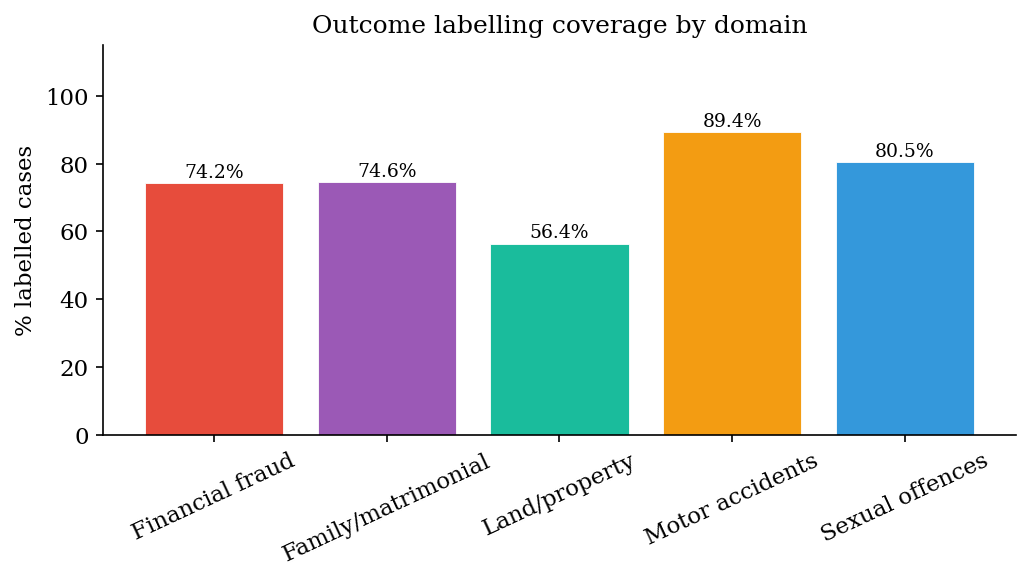
\includegraphics[width=0.92\textwidth]{figures/labelling_coverage_full.png}
  \caption{Mistral labelling coverage per bucket.}
  \label{fig:labelling_coverage}
\end{figure}

\begin{figure}[H]
  \centering
  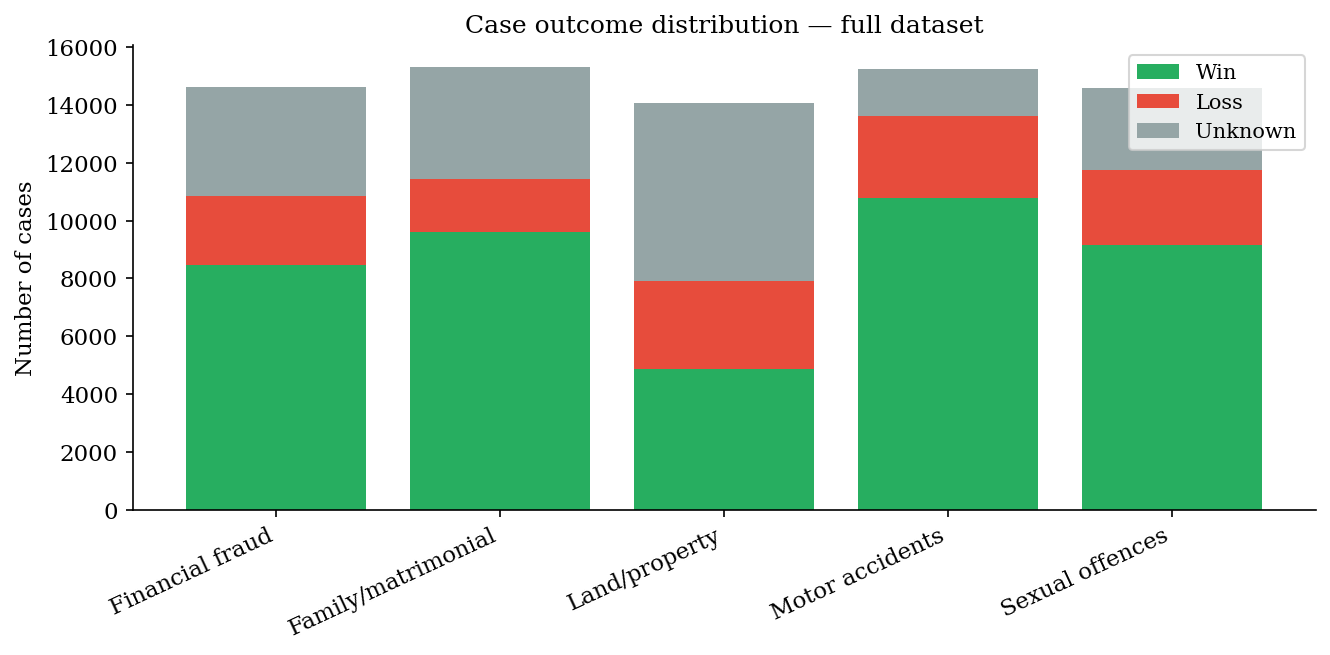
\includegraphics[width=0.92\textwidth]{figures/outcome_distribution_full.png}
  \caption{Outcome label distribution per bucket.}
  \label{fig:outcome_distribution}
\end{figure}

\section{Multi-Hearing Merging}
\label{sec:multi_hearing_merging}

\subsection{The Problem}

A single legal matter frequently produces more than one judgment
document: interim orders, remands, partial disposals, and the final
decision may all be published as separate PDFs with distinct
Indian-Kanoon-style filenames that nonetheless refer to the same case.
If these hearing files are fed into the graph independently, three
things go wrong:

\begin{enumerate}
  \item duplicate \textsc{Case} nodes for what is actually one dispute
    inflate the node count and double-count outcomes;
  \item the outcome label of the final hearing is not propagated to the
    earlier hearings, so the training signal is noisy; and
  \item cross-case structural signals (shared parties, statutes, and
    counsel across hearings) are double-counted as if they were
    independent observations.
\end{enumerate}

\subsection{Merge Strategy}

The merging pipeline lives under
\texttt{Thesis\_FINAL\_DATA/TIMELINE} and
\texttt{DATA\_SET\_BUILDER\_AND\_EXPLORER/Timeline\_Maker}. Per bucket,
filenames are parsed into a \texttt{(title,\ hearing\_date)} tuple; the
latest hearing becomes the \emph{final} case, and every older hearing
with the same title is \emph{folded} into that final case's JSON. The
fold step either appends the older document's text under a
\texttt{prior\_hearings} block (when the final document does not
already contain that text) or is skipped when the final document
already subsumes it. Every merge is logged in a per-bucket
\texttt{report.json} so the operation is auditable and reversible.

The scale of the fold is non-trivial but concentrated:

\begin{table}[H]
  \centering
  \small
  \begin{tabular}{lrrrrr}
    \toprule
    Bucket & Inputs & Final cases & Folded in & Appended & Already contained \\
    \midrule
    Family \& Matrimonial & 15{,}800 & 15{,}306 & 493 & 490 & 3 \\
    Financial Fraud & 15{,}014 & 14{,}615 & 399 & 396 & 3 \\
    Land \& Property & 14{,}324 & 14{,}051 & 251 & 242 & 9 \\
    Motor Accidents & 15{,}271 & 15{,}236 & 32 & 30 & 2 \\
    Sexual Offences & 15{,}532 & 14{,}596 & 936 & 932 & 4 \\
    \midrule
    \textbf{Total} & \textbf{75{,}941} & \textbf{73{,}804} & \textbf{2{,}111}
      & \textbf{2{,}090} & \textbf{21} \\
    \bottomrule
  \end{tabular}
  \caption{Multi-hearing merge statistics. 2{,}111 older hearing
  documents across the five buckets were folded into 2{,}090 merged
  final-case JSONs; the remaining 21 were already fully contained in
  the final hearing.}
  \label{tab:merge_stats}
\end{table}

Sexual-offences matters fold most aggressively, which is consistent with
their tendency to generate multiple remand and bail-stage orders before
a final judgment; motor-accidents matters fold least, because the
compensation process terminates in one tribunal order more often than
it does in the other buckets.

\section{Technology Stack}

The pipeline is entirely Python-based. NER, RR, and summarisation run
on top of \texttt{opennyai} with spaCy~3.2.4 and CUDA-enabled PyTorch
and CuPy, provisioned via the pinned micromamba environment
\texttt{fixed\_gpu\_opennyai\_final}. Outcome labelling uses a Mistral
model invoked through a batched client script. Multi-hearing merging is
implemented with \texttt{merge\_cases.py} and \texttt{merge\_cases\_v2.py}
under the \texttt{Timeline\_Maker} module. Graph construction is built
on \texttt{torch\_geometric}'s \texttt{HeteroData}, with text
embeddings produced by the \texttt{BAAI/bge-m3} sentence-transformer
model running multi-process on GPU and cached per bucket. Training,
ablation, and analysis scripts live under the \texttt{section\_GNN}
module.
